% -*- coding: utf-8; -*-

\chapter{Geração Semiautomática}
\label{gordon}

	Kindlmann e Durkin foram uns dos primeiros a gerar funções de transferência para visualizar as fronteiras de um volume de dados. Apesar de ter sido publicado há quase 20 anos e de possuir alguns pontos fracos já estudados por outros, seu trabalho ainda é o mais equilibrado no quesito \quote{Geração automática \textit{X} Controle do usuário}. Isso deve-se ao fato de que seu método gera bons resultados com funções de transferência 1D, que são naturalmente mais intuitivas ao usuário. Além disso, exige intervenção mínima do usuário para gerar a FT, ao mesmo tempo que permite um controle fino sobre como a fronteira deve ser apresentada visualmente. Por esse motivo, este trabalho foi escolhido como base para a pesquisa e desenvolvimento dessa dissertação e será apresentado neste Capítulo em 3 seções. A seção~\ref{gordon.bound} define o conceito de fronteira e explica como identificá-las. A obtenção do modelo matemático que gera a função de transferência 1D e 2D pode ser encontrada na seção~\ref{gordon.ft}. Por fim, o método é avaliado juntamente com alguns resultados na seção~\ref{gordon.aval}.
	
\section{Detecção de fronteiras}
\label{gordon.bound}
	\textit{Kindlmann e Durkin}~\cite{gordon} partem da premissa de que todos os materiais representados no volume de dados possuem propriedades físicas homogêneas. Dessa forma, toda fronteira seria caracterizada por uma variação abrupta na intensidade lida do volume e poderia ser representada pela função degrau. No entanto, devido aos dispositivos responsáveis pela aquisição de dados, as fronteiras são comumente borradas com uma resposta gaussiana na frequência. Por esse motivo, o comportamento de uma fronteira em um volume de dados é melhor representado pela convolução da função degrau com uma gaussiana. O resultado dessa convolução é a função \textit{erf()}, ou função \textit{erro}, ilustrada na Figura~\ref{fig:boundary_model}.
	
\begin{figure}[h]
	\centering
	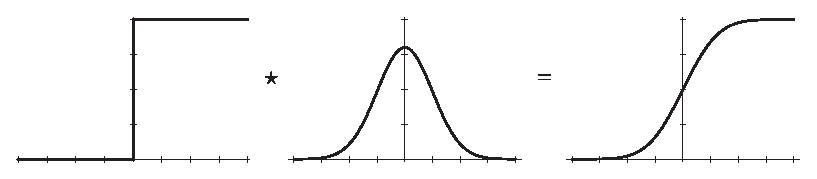
\includegraphics[width=1\textwidth]{images/g_boundary_model}
	\caption{Comportamento das funções degrau, gaussiana e erro, respectivamente~\cite{gordon}.}
	\label{fig:boundary_model}
\end{figure}

	A função \textit{erf()} é uma função contínua cuja imagem varia de $-1$ a $1$. Como uma fronteira pode variar entre quaisquer dois valores escalares contidos no volume, \textit{erf()} deve ser escalada para variar de $v_{min}$ a $v_{max}$. Assim, a função $f(x)$ que modela uma fronteira é definida pela equação~\eqref{eq:boundary}.

\begin{equation} \label{eq:boundary}
	v = f(x) = v_{min} + (v_{max} - v_{min}) \frac{1 + erf(\frac{x}{\sigma\sqrt{2}})}{2}
\end{equation} \\

	Uma outra maneira de interpretar a fronteira é como sendo uma das isosuperfícies entre $v_{min}$ e $v_{max}$. Seguindo a premissa de que a fronteira é uma variação rápida de alta intensidade, ela é melhor representada pela isosuperfície que apresenta a maior derivada. Como o vetor gradiente aponta na direção da maior taxa de variação de uma função, ele pode ser usado para caminhar entre as isosuperfícies de um volume. Assim, através da avaliação da derivada na direção do gradiente, a isosuperfície que representa corretamente a fronteira pode ser obtida.
	
\begin{figure}[h]
	\centering
%	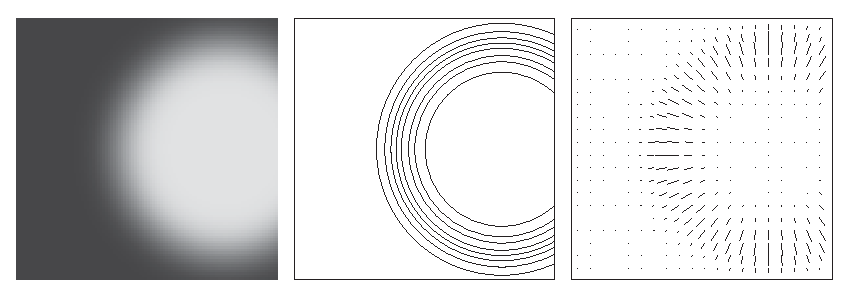
\includegraphics[width=1\textwidth]{images/grad}
	\subfigure[Intensidades]{
		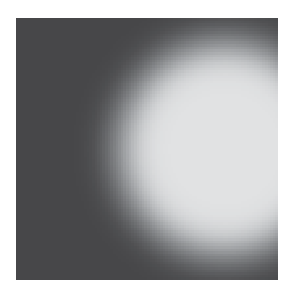
\includegraphics[width=0.3\textwidth]{images/g_cilynder}
		\label{fig:g_isosurfaces_a}
	}
	\subfigure[Isosuperfícies]{
		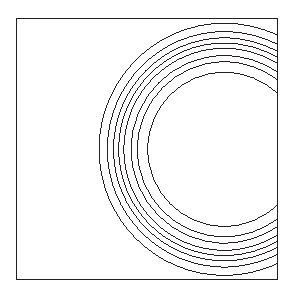
\includegraphics[width=0.3\textwidth]{images/g_isosurfaces}
		\label{fig:g_isosurfaces_b}
	}
	\subfigure[Vetores gradiente]{
		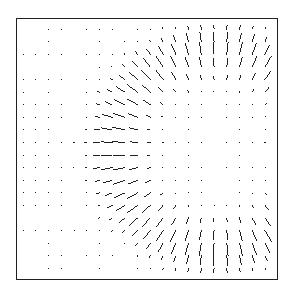
\includegraphics[width=0.3\textwidth]{images/g_grads}
		\label{fig:g_isosurfaces_c}
	}
	\caption{Visão em corte de um cilindro~\cite{gordon}.}
	\label{fig:g_isosurfaces}
\end{figure}

	A Figura~\ref{fig:g_isosurfaces}~\ref{fig:g_isosurfaces_a} mostra o corte de um volume cilíndrico, onde $v_{min}$ foi mapeado para preto e $v_{max}$ para branco. As isosuperfícies existentes entre esses valores estão ilustradas na Figura~\ref{fig:g_isosurfaces}~\ref{fig:g_isosurfaces_b}, enquanto a Figura~\ref{fig:g_isosurfaces}~\ref{fig:g_isosurfaces_c} exibe os vetores gradiente do volume. Percebe-se que os gradientes se aproximam das normais das isosuperfícies, apontando sempre para uma próxima isosuperfície, como discutido anteriormente.
		
\begin{figure}[h]
	\centering
	\subfigure[]{
		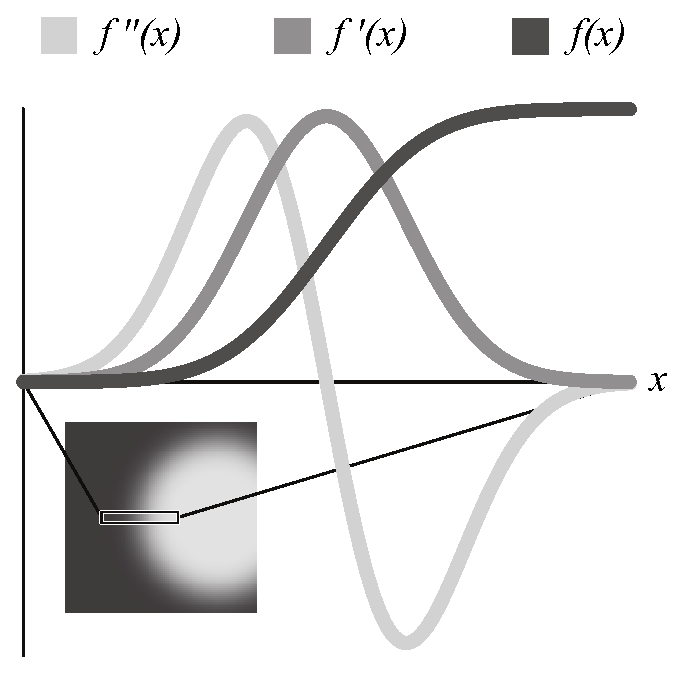
\includegraphics[width=0.4\textwidth]{images/g_functions_all}
		\label{fig:g_functions_a}
	}
	\subfigure[]{
		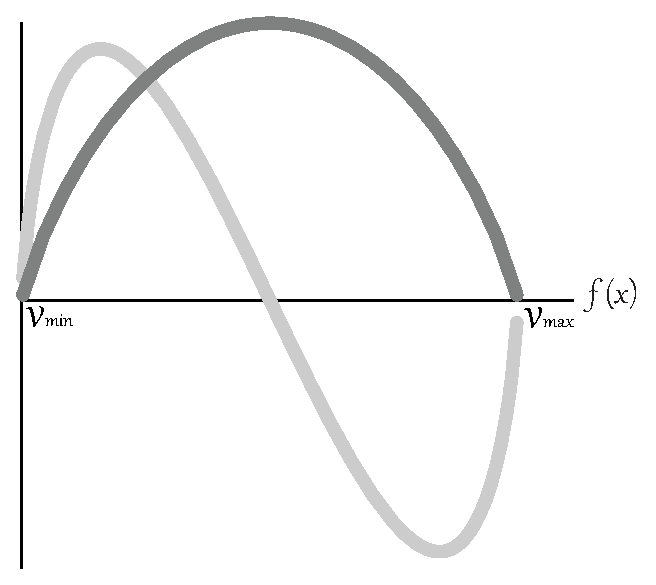
\includegraphics[width=0.4\textwidth]{images/g_functions_deriv}
		\label{fig:g_functions_b}
	}
	\subfigure{
		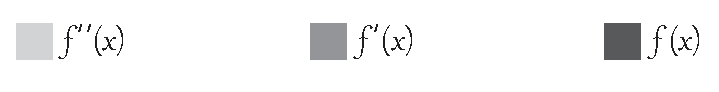
\includegraphics[width=0.5\textwidth]{images/g_functions_leg}
	}
	\caption{Comportamento das funções $f(x)$, $f'(x)$ e $f''(x)$ na direção do gradiente: \ref{fig:g_functions_a} em relação à posição, ~\ref{fig:g_functions_b} em relação ao valor escalar~\cite{gordon}.}
	\label{fig:g_functions}
\end{figure}
	
	A Figura~\ref{fig:g_functions}~\ref{fig:g_functions_a} mostra o comportamento da primeira e segunda derivadas na presença de uma fronteira. Como esperado, o ponto de maior primeira derivada e segunda derivada igual a zero identifica a posição exata da fronteira. No entanto, as curvas apresentadas só se comportam dessa forma na direção do gradiente. Isso dificulta expressar graficamente as ocorrências de fronteiras em um volume, uma vez que a direção do gradiente muda constantemente. É preciso então encontrar uma relação que identifique uma fronteira sem depender de sua posição no volume. 
	
	Uma solução simples para isso é avaliar o comportamento das derivadas em relação ao valor escalar do volume e não mais à sua posição, como mostra a Figura~\ref{fig:g_functions}~\ref{fig:g_functions_b}. Dessa forma fica mais fácil representar graficamente todas as fronteiras de um volume. Através de um histograma 2D, pode-se acumular todos os pares escalares e derivadas que ocorrem no volume. A Figura~\ref{fig:g_histo_cil} apresenta tais histogramas para o mesmo cilindro utilizado nas análises anteriores. Vê-se que as curvas da Figura~\ref{fig:g_functions}~\ref{fig:g_functions_b} aparecem nos histogramas, indicando que uma fronteira foi identificada.
	
\begin{figure}[h]
	\centering
	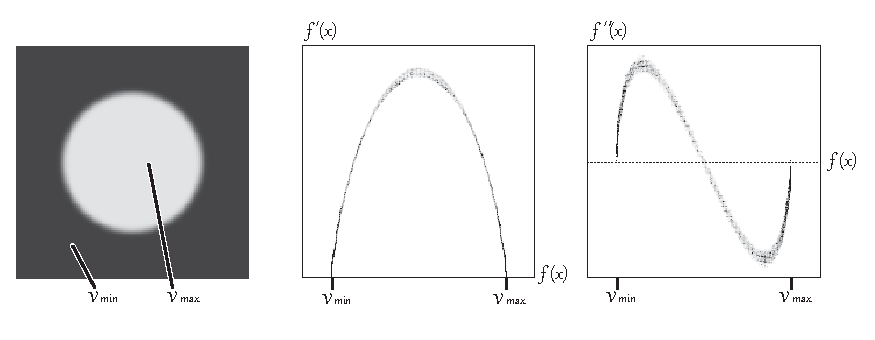
\includegraphics[width=1\textwidth]{images/g_histo_cil}
	\caption{Histogramas 2D da primeira e segunda derivada do cilindro~\cite{gordonms}.}
	\label{fig:g_histo_cil}
\end{figure}
    
\section{Geração da Função de Transferência}
\label{gordon.ft}
	A equação~\eqref{eq:boundary} deveria ser definida com 3 incógnitas, afinal o volume de dados pertence a um espaço tridimensional. No entanto, como as curvas exibidas na Figura~\ref{fig:g_functions}~\ref{fig:g_functions_a} apenas são válidas na direção do gradiente, optou-se por mantê-las com apenas uma incógnita a fim de simplificar sua leitura. Portanto, ressalta-se que a coordenada $x$ não é alinhada a um eixo do volume, mas sim à direção do gradiente no ponto em que a função $f(x)$ é avaliada. Da mesma forma, a direção na notação das derivadas parciais será omitida. Assim, a primeira e a segunda derivada de $f(x)$ na direção do gradiente são, respectivamente, $f'(x)$ e $f''(x)$ expressas nas equações \eqref{eq:first} e \eqref{eq:second}. \\
	
\begin{equation} \label{eq:first}
	f'(x) = \frac{v_{max} - v_{min}}{\sigma\sqrt{2\pi}}\ e^{-\frac{x^{2}}{2\sigma^{2}}}
\end{equation} \\

\begin{equation} \label{eq:second}
	f''(x) = -\frac{x(v_{max} - v_{min})}{\sigma^{3}\sqrt{2\pi}}\ e^{-\frac{x^{2}}{2\sigma^{2}}}
\end{equation} \\

	A função $f'(x)$ é uma gaussiana cujo desvio padrão é $\sigma$. Como a gaussiana tem pontos de inflexão em $\pm\sigma$, isso implica que $f''(x)$ atinge seus pontos extremos também em $\pm\sigma$. Observa-se pela Figura~\ref{fig:g_functions}~\ref{fig:g_functions_a} que $2\sigma$ aproxima a distância entre $v_{max}$ e $v_{min}$, servindo assim como \quote{espessura} da fronteira. Cada volume possuirá um $\sigma$ diferente, que pode ser calculado uma vez que se saiba os valores máximos de $f'(x)$ e $f''(x)$. A partir do cálculo de $\sigma$ é possível extrair $x$ relacionando $f'(x)$ e $f''(x)$, como mostram as equações \eqref{eq:sigma} e \eqref{eq:x}.
	\\
	
\begin{equation} \label{eq:sigma}
	\sigma = \frac{f'(0)}{\sqrt{e}f''(-\sigma)}
\end{equation} \\

\begin{equation} \label{eq:x}
	x = -\frac{\sigma^{2}f''(x)}{f'(x)}
\end{equation} \\

	Isolar $x$ é importante pois ele é mais que uma posição do volume na direção do vetor gradiente. A posição indicada por $x$ é perpendicular à fronteira e relativa ao centro desta mesma fronteira, ou seja, $|x|$ é a distância ao centro da fronteira. Agora fica mais fácil designar uma opacidade para cada voxel do volume, basta relacionar sua transparência de acordo com a sua distância à fronteira.
	
	A função par que decresce linearmente de $1$ a $0$ no intervalo $[0,\sigma]$ e permanece $0$ em $[0, \infty]$ é talvez a forma mais intuitiva de relacionar a transparência com a distância $x$ à fronteira. O volume se torna completamente opaco apenas nos pontos onde há ocorrência do centro exato de uma fronteira e vai perdendo essa opacidade linearmente até atingir uma região homogênea. Contudo, um ganho relevante é obtido se for designado ao usuário a tarefa de definir uma função de opacidade $b(x)$, responsável por descrever a relação \quote{distância X opacidade} descrita anteriormente.
	
	Através de $b(x)$ o usuário ganha um controle fino sobre o render final do volume, pois cabe a ele dizer como a fronteira deve ser visualizada. A Figura~\ref{fig:ig:bx} mostra como diferentes opções de $b(x)$ podem afetar a visualização final. Nesse exemplo o volume é composto por duas esferas concêntricas de raios distintos. Percebe-se que apenas variando a função de opacidade é possível alternar entre: visualizar apenas a esfera de fora ou ambas, visualizar toda a fronteira ou apenas o lado interior da esfera que compõe a fronteira, ou até mesmo decidir entre uma transição suave ou abrupta.
	
\begin{figure}[h]
	\centering
	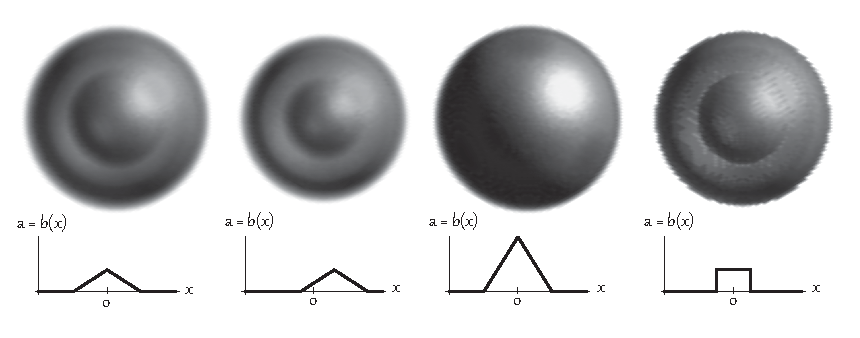
\includegraphics[width=1\textwidth]{images/g_bx}
	\caption{O impacto de diferentes funções de opacidade $b(x)$ na visualização de duas esferas concêntricas~\cite{gordon}.}
	\label{fig:g_bx}
\end{figure}

	Esse controle é especialmente importante quando as fronteiras de um volume não se comportam da forma ideal. Por exemplo, uma fronteira com o crescimento mais acentuado de um lado fará com que a distância $x$ seja deslocada. Neste caso, a correção desse deslocamento se torna muito mais simples se feita em $b(x)$ ao invés de $f(x)$. O usuário continua livre de ter que inspecionar o volume em busca da fronteira, mesmo que o método seja apenas capaz de indicar sua proximidade.
	
\subsection{Função de Transferência 1D}
\label{gordon.1d}
	Com a premissa de que os materiais têm propriedades físicas homogêneas e o modelo definido na seção~\ref{gordon.bound}, pode-se assumir também que os valores do volume na fronteira são sempre os mesmos e que, na média, um fronteira pode ser atribuída a um valor escalar. Isso fica claro na Figura~\ref{fig:g_functions}~\ref{fig:g_functions_b} onde foi encontrado um padrão para identificar as fronteiras em função de $v$.
	
	A equação~\eqref{eq:x} reescrita em função de $v$ é apresentada na equação~\eqref{eq:pv}, cujo significado pode ser interpretado como a distância média com que os voxels de valor $v$ se encontram da fronteira mais próxima a eles. Nela, $g(v)$ indica a média da primeira derivada na direção do gradiente sobre todas as posições $x$ do volume de valor $v$. Da mesma forma, $h(v)$ indica a média da segunda derivada na direção do gradiente sobre todas as ocorrências de $v$. %TODO Comentar que g(v) e h(v) podem ser extraídos das fativas 'v' do histograma 3D
	%TODO explicar Gtresh
	\\	

\begin{equation} \label{eq:pv}
	p(v) = -\frac{\sigma^{2}h(v)}{max(g(v) - g_{tresh}, 0)}
\end{equation} \\

	Como explicado previamente, o $\sigma$ é obtido em função dos valores extremos de $f'(x)$ e $f''(x)$. No entanto, apesar de ser uma característica do volume e, portanto, constante, ele também precisa ser reformulado em função de $v$. O cálculo de $\sigma$ utilizando os máximos globais do volume pode distorcer todas as distâncias médias, por causa de ruído. Assim, os valores extremos utilizados devem ser os máximos dentre os valores médios: $g(v)_{max}$ e $h(v)_{max}$, como na equação~\eqref{eq:sigmav}. Uma forma mais equilibrada de obter o $\sigma$ é utilizar também o extremo mínimo da segunda derivada direcional, como demonstrado na equação~\eqref{eq:sigmav2}. \\
	
\begin{equation} \label{eq:sigmav}
	\sigma = \frac{g(v)_{max}}{\sqrt{e}\ h(v)_{max}}
\end{equation} \\

\begin{equation} \label{eq:sigmav2}
	\sigma = \frac{2\ g(v)_{max}}{\sqrt{e}\ (h(v)_{max} - h(v)_{min})}
\end{equation} \\

	A função $b(x)$ definida pelo usuário continua conceitualmente correta. Contudo, uma simples transformação de notação precisa ser feita, afinal deseja-se designar opacidade em função de $v$ e no entanto, a função responsável por definir opacidade está em função de $x$. Define-se então a equação~\eqref{eq:alpha} \\
	
\begin{equation} \label{eq:alpha}
	\alpha(v) = b(p(v))
\end{equation}

	%TODO INSERIR RESULTADOS
    
\subsection{Função de Transferência 2D}
\label{gordon.2d}
    Desenhar uma função de transferência 2D é ainda mais difícil que uma 1D. Contudo, obter funções 2D pode ser desejável. Segundo \textit{Kindlmann e Durkin}~\cite{gordon}, definir a opacidade em função do valor escalar e da primeira derivada pode gerar melhores resultados. Isso porque em volumes mais complexos pode haver sobreposição nos intervalos de fronteiras distintas. Os histogramas 2D revelam bem essas sobreposições, uma vez que os arcos se tocam quando isso ocorre. Um exemplo desse problema é visto na Figura~\ref{fig:}.
    
    Contudo, o método proposto até aqui pode ser facilmente estendido para uma versão 2D... SIGMA NÃO MUDA, EXPLICA H(V,G) E MOSTRA A EQUAÇÃO NOVA, DAI DIZ QUE "NOVAMENTE...POR AJUSTE NA NOTAÇÃO" E ENTÃO MOSTRA A(V, G).
    
\section{Avaliação do método}
\label{gordon.aval}    
    Atacar treshold do gordon, apresentando minha solução. Mas sem criticar de forma negativa.
    
    Comentar 2ª derivada média.
    
    Como bem ressaltado por \textit{Sereda et al.}~\cite{sereda1}, é comum esperar que aumentar a dimensão da função de transferência vá trazer melhores resultados e eliminar a sobreposição de fronteiras, mas frequentemente esse não é o caso. Por esse motivo, a intuitividade em assimilar e manipular uma FT 1D foi o que motivou
    
    
    Principalmente se analisado segundo a versão 1D de sua função de transferência. Seu método trás bons resultados sem exigir intervenção do usuário. E no caso da versão 1D a interface para ser gerada e ao mesmo tempo, a versão 1D é intuitiva
    
    
    Como visto no Capítulo~\ref{related}, o trabalho de \textit{Kindlmann e Durkin}~\cite{gordon} é o que menos exige iteração do usuário para detectar fronteiras automaticamente e, ao mesmo tempo, permitindo que este possa controlar a função de transferência gerada.
    Faça uma apresentação do método....extende o trabalho relacionado + introdução e (talvez) emende nesse início de deteção de fronteira...(talvez não rs).